\documentclass[letterpaper,twocolumn,10pt]{article}
\usepackage{usenix_zh}
\usepackage{amsmath,amssymb}
\usepackage{booktabs,multirow,makecell,tabularx,array}
\usepackage{graphicx}
\usepackage{subcaption}
\usepackage{enumitem}
\usepackage{caption}
\captionsetup{font=small}
\captionsetup[subfigure]{font=small}

\renewcommand{\figurename}{图}
\renewcommand{\tablename}{表}
\renewcommand{\abstractname}{摘要}
\renewcommand{\refname}{参考文献}

\newcommand{\sys}{Catalyzer}
\newcommand{\etal}{\textit{et al.}}
\newcommand{\figref}[1]{图~\ref{#1}}
\newcommand{\tabref}[1]{表~\ref{#1}}
\newcommand{\secref}[1]{第~\ref{#1}~节}
\newcommand{\para}[1]{\paragraph{#1}}

\title{\sys{}：面向 Serverless 计算的亚毫秒级启动与免初始化引导}

\author{
Dong Du$^{1,2}$ \quad Tianyi Yu$^{1,2,3}$ \quad Yubin Xia$^{1,2}$ \quad Binyu Zang$^{1,2}$\\
Guanglu Yan$^{3}$ \quad Chenggang Qin$^{3}$ \quad Qixuan Wu$^{3}$ \quad Haibo Chen$^{1,2}$\\[0.5em]
$^{1}$上海交通大学可扩展计算与系统上海市重点实验室\\
$^{2}$上海交通大学并行与分布式系统研究所\\
$^{3}$蚂蚁金服
}

\date{}

\begin{document}
\pagestyle{empty}
\maketitle

\begin{abstract}
Serverless 计算以较高的开发效率、良好的弹性以及按需付费能力而受到广泛关注。
为了兑现这些优势，Serverless 沙箱系统必须同时满足两个目标：其一是实例之间的强隔离，其二是足够低的启动时延，以避免冷启动显著损害用户体验。
基于虚拟化的沙箱能够提供强隔离，但沙箱本身与应用程序的初始化都会带来不可忽略的启动开销。
现有系统大多是面向应用无关的通用优化，只能通过裁剪 Hypervisor 或客体内核来缩短沙箱初始化路径，却无法消除占比更高的应用初始化成本。

本文提出 \sys{}，一种兼具强隔离与极低启动时延的 Serverless 沙箱设计。
\sys{} 不再从零启动函数实例，而是从一个结构良好的检查点镜像中恢复虚拟化沙箱实例，从而把初始化移出关键路径，实现免初始化引导（init-less booting）。
为了进一步加速恢复，\sys{} 对用户态内存状态和系统状态都采用按需恢复；同时，我们提出新的操作系统原语 \emph{sfork}（sandbox fork），可以直接复用一个正在运行的模板沙箱状态，以进一步降低启动时延。
从根本上看，\sys{} 通过状态复用消除了初始化成本，因此可以为多种 Serverless 函数提供通用优化。

评估结果表明，\sys{} 能将启动时延降低数个数量级，在最佳情况下达到亚毫秒级，并能显著改善真实工作负载的端到端时延。
\sys{} 已在蚂蚁金服内部落地，文中还总结了工业开发中的若干实践经验。
\end{abstract}

\vspace{0.3em}
\noindent\textbf{关键词：}Serverless 计算；启动时延；检查点与恢复；操作系统

\section{引言}\label{sec:intro}
Serverless 计算已经成为云计算中的重要范式之一，它把开发者从服务器运维与资源编排中解放出来，并已经被 Amazon Lambda、IBM Cloud Functions、Microsoft Azure Functions 和 Google Cloud Functions 等平台广泛采用~\cite{r2,r1,r3,r7}。
在 Serverless 模型中，函数是计算的基本单位：当服务请求到达时，平台会分配一个短生命周期的执行沙箱，并实例化用户定义的函数处理该请求。
这种模型把动态管理云资源的责任交给云厂商，使开发者能够更专注于业务逻辑，同时也让云厂商更高效地利用资源。

承载函数的执行沙箱通常是容器、虚拟机，或者近年来提出的轻量级虚拟化设计~\cite{r1,r20,r44,r6,r8,r19,r35,r37,r41,r45}。
容器虽然轻量，但共享内核带来了明显的隔离风险；虚拟机隔离性更好，却往往过于笨重，不适合频繁创建的 Serverless 实例。
类似 gVisor 与 Firecracker 的轻量级虚拟化系统通过定制主机-客体接口在性能、资源管理和隔离之间取得了更好的平衡~\cite{r8,r6}。

\begin{figure}[t]
  \centering
  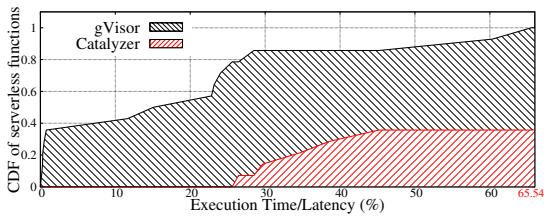
\includegraphics[width=0.95\linewidth]{images/89157301d724057ee3201f62f8ea476f4b69e1933f1276030ff6d68c08e71db8.jpg}
  \caption{Serverless 场景中“执行时间/总时延”比例的分布。对于 gVisor 上测试的函数，所有样例都无法超过 65.54\%，大多数甚至低于 30\%，说明冷启动成本主导了总体时延。}
  \label{fig:ratio}
\end{figure}

低时延执行 Serverless 函数对用户体验至关重要~\cite{r21,r24,r28,r32,r38}，但这仍是虚拟化沙箱设计中的关键难题。
为说明问题的严重性，我们对 DeathStar 微服务基准、一个电商微服务场景以及图像处理函数进行了端到端测量，并将总时延拆分为执行部分和启动部分。
如 \figref{fig:ratio} 所示，在 gVisor 上测试的 14 个函数中，有 12 个函数的“执行时间/总时延”比例甚至不足 30\%，说明启动过程已经成为整体时延的主导因素。

现有基于虚拟机的沙箱系统大多通过定制 Hypervisor 来缩短启动路径，例如 Firecracker 能在大约 100ms 内启动 microVM 与一个精简 Linux 内核~\cite{r6,r8,r37}。
然而，这类方案无法消除应用层初始化开销，例如 JVM 启动、Python 解释器初始化等。
我们对 5 种编程语言编写的 Serverless 函数进行研究后发现，绝大部分启动时延其实都来自应用初始化，而不是沙箱初始化本身，这构成了本文的 \emph{洞见 I}。

基于这一发现，本文提出 \sys{}，其核心思想是在关键路径上不再执行初始化，而是从结构良好的检查点镜像直接恢复实例。
这一设计还建立在两个额外洞见之上。
首先，函数在真正执行用户请求时，通常只会访问初始化阶段涉及的内存页和文件中的很小一部分；因此，用户态状态和系统状态都可以按需恢复，这构成 \emph{洞见 II}。
其次，同一函数的多个实例在完成初始化后拥有极为相似的状态，因此运行中的实例状态也可以被复用，从而派生出新的实例，这构成 \emph{洞见 III}。
为此，\sys{} 一方面对用户级状态与系统状态都采用按需恢复，另一方面提出新的操作系统原语 \emph{sfork}（sandbox fork），直接复用运行中模板沙箱的状态，以进一步缩短启动路径。

我们基于 gVisor 实现了 \sys{}，并在微基准与真实应用上进行了系统评估。
结果表明，在最佳情况下，\sys{} 可把 C 语言 HelloWorld 函数的启动时延降到 \(<1\,\mathrm{ms}\)；对于 Java SPECjbb，启动时延可降到 \(<2\,\mathrm{ms}\)，相比基线 gVisor 提升可达约三个数量级。
我们还在蚂蚁金服的服务器环境中验证了其效果，并总结了工业实践经验。

本文的主要贡献如下：
\begin{itemize}[leftmargin=1.2em]
  \item 对 Serverless 计算中的启动时延开销进行了系统化分析，明确指出应用初始化是主要瓶颈；
  \item 提出了通用的免初始化启动设计，并通过按需恢复与 \emph{sfork} 同时优化冷启动、温启动和热启动；
  \item 在 Google gVisor 上完成了 \sys{} 的实现，并验证了该设计在最先进虚拟化沙箱上的可行性；
  \item 通过微基准与真实 Serverless 工作负载的评估，证明了 \sys{} 的高效性与工程可落地性；
  \item 总结了 \sys{} 在工业环境部署中的经验与启示。
\end{itemize}

\section{Serverless 函数启动开销分解}\label{sec:breakdown}
本节在不同系统沙箱（gVisor、Firecracker、Hyper Container 与 Docker）和不同语言运行时上，对 Serverless 平台的启动时延进行评估与分析，并据此说明为什么 Serverless 函数应该采用免初始化方式执行。

\subsection{背景}\label{sec:background}
\para{Serverless 平台工作流。}
在 Serverless 平台中，开发者提交一个函数供平台执行。
本文用 \emph{handler function} 表示真正的用户函数，它可以用不同语言编写。
离线阶段，平台会把 handler 与一个 \emph{wrapper} 一起编译；wrapper 负责完成初始化，并在适当时机调用 handler。
包装后的程序在沙箱中安全执行，沙箱可以是容器或虚拟机~\cite{r5,r40,r6,r8,r10}。
每台服务器上通常有一个守护进程式网关程序，它接收“调用函数”请求，并以两个参数启动沙箱：配置文件以及包含包装程序和运行时库的 rootfs。
这两个参数遵循 OCI 规范~\cite{r12}，因此与多数现有 Serverless 平台兼容。

\para{以 gVisor 为例。}
本文用 gVisor 作为分析、实现与评估的代表案例，目标是在这类基于虚拟化的沙箱上实现亚毫秒级启动。
在一次函数调用中，首先需要准备沙箱。
对 gVisor 来说，这一阶段包括四个主要步骤：解析配置、分配虚拟化资源（如 vCPU 与客体内存区域）、挂载根文件系统，以及初始化客体内核，如 \figref{fig:gvisor-boot} 所示。
在 gVisor 中，客体内核由两个用户态进程协作实现：一个沙箱进程负责设置虚拟化资源（例如扩展页表 EPT）并准备客体内核；另一个 I/O 进程依据配置文件挂载 rootfs。
实验表明，仅沙箱初始化一项就在 gVisor 中需要约 22.3ms，而且由于其依赖函数特定配置，像缓存这类手段很难直接消除这一成本。
文中所说的“关键路径”指的是从网关收到请求到 handler 真正可以执行的时间段，而所有非关键路径上的工作统称为 \emph{offline} 操作。

包装程序启动后，会继续完成运行时初始化并准备执行用户函数。
以 Java 为例，包装程序首先启动 JVM，加载类文件等运行时组件，然后才进入用户提供的 handler。
我们把从包装程序启动到 handler 可以执行为止的时间定义为 \emph{应用初始化时延}；后续评估将显示，这一部分往往主导总体启动成本。

\begin{figure*}[t]
  \centering
  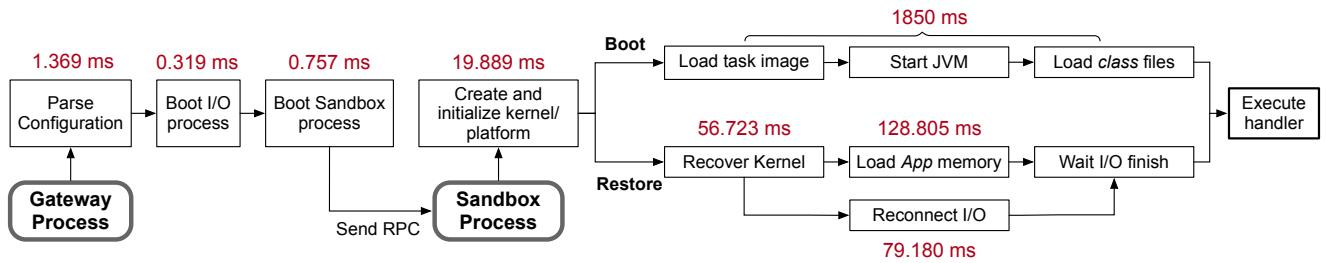
\includegraphics[width=0.95\textwidth]{images/d95f7449ffbf143f74a571c0afa8fab00b3160f503c1090139e58cd9bbda7738.jpg}
  \caption{gVisor 的启动流程。图中标注的是 Java SPECjbb 场景下各步骤的时延；Restore 路径表示使用 gVisor 原生检查点/恢复机制从镜像恢复沙箱的过程。}
  \label{fig:gvisor-boot}
\end{figure*}

\begin{figure}[t]
  \centering
  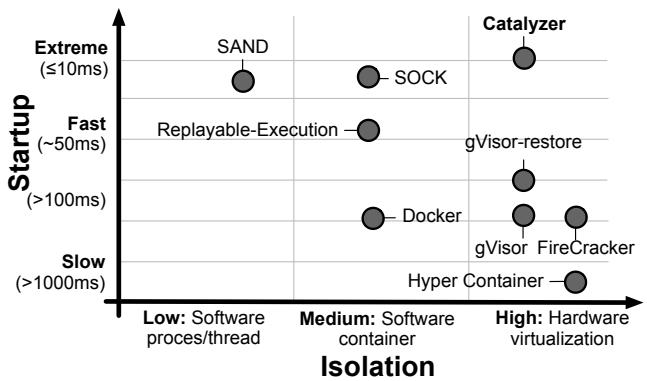
\includegraphics[width=\linewidth]{images/8228a51b1f0f1cf92023dd264858690e9cb537bbffa8f3384bcacf42ebcf6eed.jpg}
  \caption{Serverless 沙箱设计空间。\sys{} 是图中唯一同时兼顾强隔离与低启动时延的方案。}
  \label{fig:design-space}
\end{figure}

\subsection{启动优化的定量分析}\label{sec:quantitative}
\para{基于缓存的优化。}
许多系统使用缓存来优化 Serverless 启动~\cite{r17,r39,r40}。
例如，Android 中广泛使用的 Zygote 机制可通过复用已预热的 Java 运行时来快速创建应用~\cite{r14}；SOCK~\cite{r40} 把这一思想迁移到 Serverless 中，为 Python 解释器建立预热缓存；SAND~\cite{r17} 允许同一应用函数的多个实例共享装有代码和库的沙箱。
但缓存方案有两个根本问题。
第一，一台机器上可能同时承载成千上万个函数，把所有函数都缓存在内存中代价过高，实际场景中的缓存策略也很难精准设计。
第二，缓存无法解决尾时延问题，因为尾时延往往由缓存未命中时的冷启动主导。

\para{针对沙箱初始化的优化。}
除了缓存，已有沙箱系统也尝试通过系统定制来缩短初始化路径。
例如 SOCK~\cite{r40} 设计了更精简的容器，以降低沙箱准备成本。
与容器不同，基于虚拟机的沙箱能够提供更强隔离，但也引入了更多初始化成本。
围绕传统重型虚拟化系统，研究者提出了许多轻量级虚拟化技术~\cite{r6,r19,r26,r36,r37}，分别从 Hypervisor、客体内核或两者结合的角度降低性能与资源开销~\cite{r18,r23,r25,r29}。
这些工作直接推动了 gVisor 与 Firecracker 等工业系统的出现~\cite{r8,r6}。

\begin{figure}[t]
  \centering
  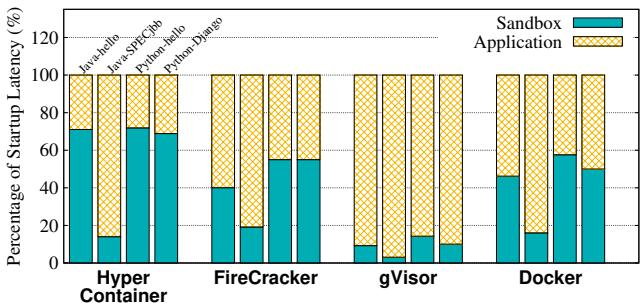
\includegraphics[width=\linewidth]{images/0fda6754aad3d502ad54da07aa835fb23cdc22bc31430d68e00926352a1c103c.jpg}
  \caption{不同工作负载上的启动时延分布。对于 Java SPECjbb 这类复杂应用，应用初始化成本占绝对主导；对于 Python Hello 这类轻量应用，沙箱初始化也有较高占比。}
  \label{fig:startup-distribution}
\end{figure}

尽管轻量级虚拟化系统的设计和实现各不相同，它们仍共享同一局限：无法消除 JVM、Python 解释器等应用初始化成本。
为定量理解这一问题，我们直接调用四种广泛使用的沙箱运行时（gVisor、Firecracker、Hyper Container 和 Docker），在不同工作负载上测量其启动时延分布，如 \figref{fig:startup-distribution} 所示。
实验只测量沙箱运行时本身，不计入容器管理等额外开销，环境与 \secref{sec:eval-env} 保持一致。

结果揭示了三个重要现象。
第一，启动成本的大头来自应用初始化，而非沙箱本身。
第二，与 C 语言相比，Java 与 Python 等高级语言的启动时延要高得多，因为它们需要先初始化语言运行时，再装载应用代码。
第三，沙箱初始化对不同工作负载相对稳定，但在 Python Hello 这类简单函数上会成为主要瓶颈。
因此，仅优化虚拟化层而不处理应用初始化，并不足以真正解决 Serverless 启动问题。

\begin{figure}[t]
  \centering
  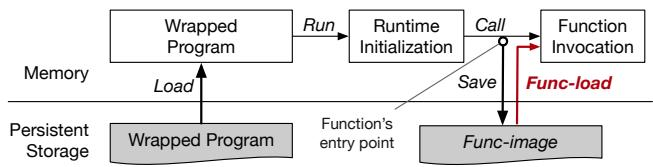
\includegraphics[width=\linewidth]{images/9fa93cbeda06c2bd78bb991fdd02c542150c78825e881e7080c51f09aefab51d.jpg}
  \caption{免初始化引导（init-less booting）的抽象流程。}
  \label{fig:initless}
\end{figure}

\para{基于检查点/恢复的优化。}
检查点/恢复（checkpoint/restore, C/R）技术可以把一个运行中沙箱的状态保存到检查点镜像中，状态既包括应用数据，也包括沙箱状态（例如虚拟化系统内部状态）。
之后，系统可从镜像中恢复出沙箱，并继续无缝执行。
Replayable Execution~\cite{r43} 利用了这一思路来降低 Java 类函数的初始化成本，并通过按需装载内存来加速容器恢复。
然而，我们的分析发现，在基于虚拟化的沙箱中，系统状态恢复本身就会带来很高的额外开销，而这是此前工作的关注盲区。

C/R 的核心好处在于：它能把应用初始化成本转换为恢复成本。
本文将这一思想概括为 \emph{免初始化引导}，如 \figref{fig:initless} 所示。
在离线阶段，系统先生成一个函数镜像（func-image），保存函数在初始化完成后的状态；在线阶段，平台只需获取这一镜像，并复用其中保存的状态即可加速后续启动。

\begin{figure}[t]
  \centering
  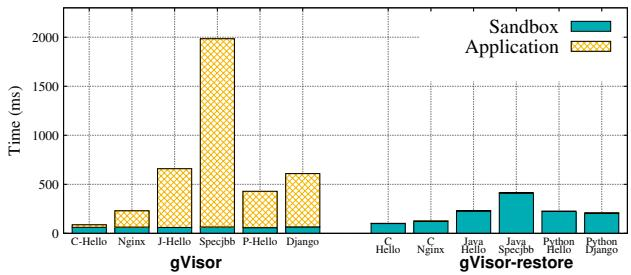
\includegraphics[width=\linewidth]{images/896c52a21da9643400eaf579d03ef12ec9194f6f4a4927394f3d2169dca5a23b.jpg}
  \caption{gVisor 与 gVisor-restore 的启动时延对比。gVisor-restore 通过 C/R 消除了应用初始化成本，但整体恢复时延依然偏高。}
  \label{fig:gvisor-restore}
\end{figure}

\para{挑战。}
传统 C/R 通过复用序列化状态来减少应用初始化成本，但它仍依赖 \emph{re-do} 操作来恢复系统状态，特别是内核中的打开文件、线程上下文等。
例如，恢复系统必须重新执行 \texttt{open()} 来重新打开先前已打开的文件。
这些 re-do 操作在虚拟化沙箱中尤为昂贵。

为了分析这一点，我们在 gVisor 提供的检查点/恢复机制基础上实现了一个免初始化启动原型，称为 gVisor-restore~\cite{r4}。
我们在 gVisor 中新增了一个系统调用，用于在函数入口点处陷入内核；所谓 \emph{func-entry point}，即函数真正处理用户请求前的最后一个位置，可以由开发者显式指定，也可以是包装程序调用 handler 之前的默认位置。
当程序执行到该位置时，系统调用会阻塞，直到检查点开始。

如 \figref{fig:gvisor-restore} 所示，gVisor-restore 的确消除了应用初始化开销，相比原始 gVisor 有 2--5 倍提升；然而它的恢复时延依然很高：Java SPECjbb 仍需约 400ms，其它场景通常也超过 100ms。
结合 \figref{fig:gvisor-boot} 可以看到，gVisor-restore 在客体内核恢复上仍花费约 135.9ms，其中既包括线程等非 I/O 系统状态的恢复，也包括文件等 I/O 状态的重连。
对于可复用的应用内存状态，gVisor 还会先压缩镜像、恢复时再解压、反序列化并装载到内存，这在 SPECjbb 场景中又带来了 128.8ms 开销。
在该案例里，系统需要恢复超过 37{,}838 个对象，并装载约 200MB 的内存数据。

综上，容器场景下仅做按需分页是不够的；在虚拟化沙箱中，系统状态恢复同样必须被纳入优化范围。

\subsection{概览}\label{sec:overview}
上述分析促使我们提出 \sys{}：一种面向虚拟化沙箱的免初始化启动设计，它通过新的按需恢复技术克服传统恢复路径中的高时延问题。

\begin{figure}[t]
  \centering
  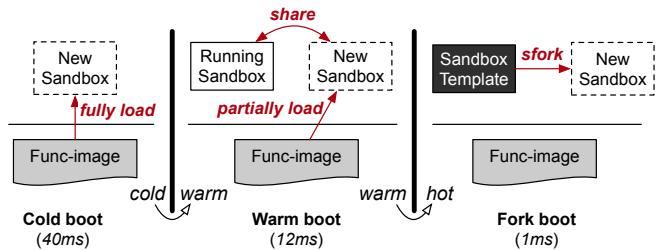
\includegraphics[width=\linewidth]{images/ef1d485c18f5fb10bd2c68fef425bbdaabd4c8df6420d0c060f5c9dca6867708.jpg}
  \caption{\sys{} 概览。\sys{} 将检查点/恢复与沙箱 fork 结合起来，同时优化冷启动与热启动。}
  \label{fig:overview}
\end{figure}

如 \figref{fig:overview} 所示，\sys{} 定义了三种启动模式：冷启动、温启动与 fork 启动。
冷启动指平台必须从函数镜像恢复出一个新沙箱；温启动指该函数已有实例在运行，此时 \sys{} 可以共享在内存中的状态加速恢复；fork 启动则依赖专门的模板沙箱（template sandbox），该模板已经完成初始化，可直接派生新实例，因此是一种更积极的热启动机制~\cite{r11,r40}。
与传统热启动不同，fork 启动可以从单一模板扩展出任意数量的新实例，而不会像缓存一样受到缓存容量限制。

\sys{} 采用混合方案：一方面利用基于 C/R 的免初始化恢复实现冷启动和温启动；另一方面通过新的 OS 原语 \emph{sfork} 直接复用模板沙箱状态，从而实现更快的 fork 启动。
鉴于函数在执行阶段通常只访问初始化阶段涉及资源的一小部分，\sys{} 在冷启动和温启动中都采用按需恢复来优化应用状态与系统状态；而对于频繁调用的热点函数，fork 启动虽然会增加一定内存占用，但能够带来更低的时延。

\section{按需恢复}\label{sec:ondemand-restore}
恢复阶段的成本主要来自两部分：一是应用与系统状态的解压、反序列化以及装载；二是为重建系统状态所必须执行的 re-do 操作，例如线程上下文、虚拟化沙箱以及 I/O 连接的恢复。
\sys{} 的总体思想是把恢复过程拆成三个阶段：离线准备、关键路径恢复以及按需恢复。
像解压和大部分反序列化这样的工作尽量前移到检查点阶段完成；应用状态加载和 I/O 相关系统状态恢复则延后到真正需要时再做。
因此，关键路径只保留不可回避的非 I/O 系统状态恢复。

为此，\sys{} 提出四项关键技术：覆盖内存（overlay memory）、分离式状态恢复、按需 I/O 重连以及虚拟化沙箱 Zygote。
它们分别对应应用状态装载、系统元数据恢复、I/O 状态恢复和沙箱构建四个方面的瓶颈。

\begin{figure*}[t]
  \centering
  \begin{subfigure}[t]{0.31\textwidth}
    \centering
    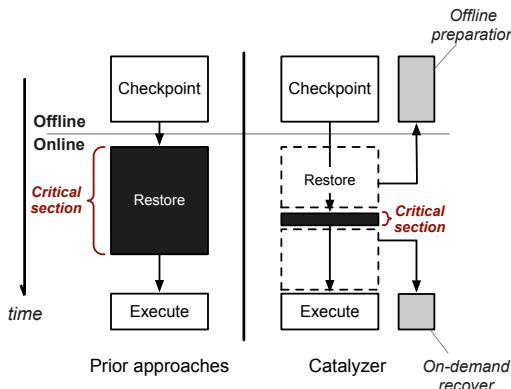
\includegraphics[width=\linewidth]{images/09a98ccbebad1e63428996a52f98674d30bab169cfd61ffee9895a184f38fa88.jpg}
    \caption{与已有方案对比。}
  \end{subfigure}\hfill
  \begin{subfigure}[t]{0.31\textwidth}
    \centering
    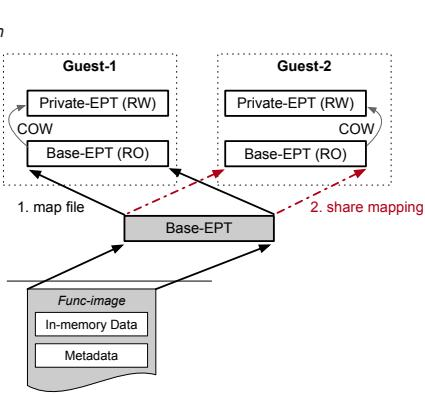
\includegraphics[width=\linewidth]{images/37e78c61f648cebc84980300b13a6e05ef022367f47b4e887c85e7045c173bbf.jpg}
    \caption{覆盖内存。}
  \end{subfigure}\hfill
  \begin{subfigure}[t]{0.31\textwidth}
    \centering
    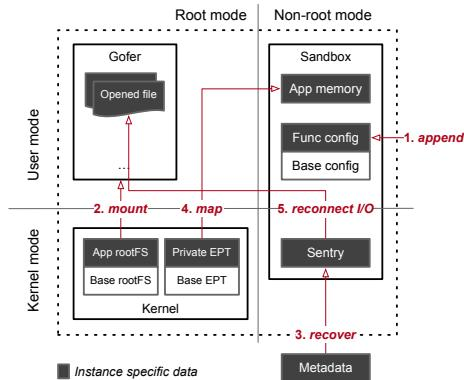
\includegraphics[width=\linewidth]{images/bdfda5a2ae412253c138d494bb41c58f0fe2067db003ba79f5096a310919575a.jpg}
    \caption{运行流程。}
  \end{subfigure}
  \caption{按需恢复。与已有方案相比，\sys{} 把大量工作转移到离线阶段，并通过按需恢复消除关键路径上的大部分开销；覆盖内存使函数镜像可直接映射到内存以构建 Base-EPT，并通过写时复制在不同实例之间共享；整体流程展示了 gVisor 沙箱如何利用按需恢复被实例化。}
  \label{fig:ondemand}
\end{figure*}

\subsection{覆盖内存}\label{sec:overlay-memory}
覆盖内存是一种面向按需应用状态装载的内存抽象，它基于文件映射与写时复制实现，如 \figref{fig:ondemand} 所示。
它允许同一函数的多个沙箱共享一个“基础内存映射”（base memory mapping），同时依靠内存级写时复制保证实例之间的隔离。

覆盖内存要求函数镜像是结构良好的：其中应用状态必须未压缩、按页对齐，并可直接映射。
在冷启动时，\sys{} 通过一次 \texttt{mmap} 直接把函数镜像载入内存；系统为每个沙箱维护两层 EPT：上层为 Private-EPT，仅该实例可见；下层为 Base-EPT，可只读共享。
在温启动时，新实例可以直接共享已有实例的 Base-EPT，从而省去昂贵的文件装载成本。

硬件执行时，系统通过合并 Private-EPT 与 Base-EPT 来构造最终的 EPT：若 Private-EPT 中存在有效项，则使用其映射，否则回退到 Base-EPT。
Base-EPT 只读、可共享，因此能通过 \texttt{mmap} 被多个实例继承；一旦某页发生写访问，系统就通过写时复制在 Private-EPT 中建立私有页，既保证了效率，也保证了隔离。

\subsection{分离式状态恢复}\label{sec:separated-recovery}
传统 C/R 依赖系统状态的元数据对象来执行 re-do 操作，例如线程链表、定时器、挂载点等。
这些元数据在保存前会被序列化，恢复时再逐个反序列化。
对于使用高级语言实现的沙箱（例如用 Go 编写的 gVisor）而言，这一过程代价尤其高昂：高级语言的运行时抽象掩盖了对象的底层布局，即便借助 Protocol Buffers 这类序列化工具~\cite{r16}，恢复时仍需要逐对象处理。
在 SPECjbb 场景中，仅这一过程就要处理 37{,}838 个对象，并消耗超过 50ms。

为了解决这个问题，\sys{} 提出 \emph{分离式状态恢复}：把“反序列化”与“系统状态真正恢复”解耦。
在离线阶段，\sys{} 会先把离散的内存对象重新组织为连续内存块，使其可通过 \texttt{mmap} 直接映射回内存，而无需逐对象反序列化；随后，把对象中的指针字段清零并替换为占位符，并用一张 \emph{关系表} 记录所有“指针所在偏移 $\rightarrow$ 指针目标偏移”的映射关系。
元数据对象与关系表共同构成一种“部分反序列化”的对象表示。

有了这种表示之后，恢复流程被拆成两个阶段：第一阶段使用覆盖内存把部分反序列化对象与关系表直接映射到内存；第二阶段依据关系表重建对象间引用关系，并并行恢复非 I/O 系统状态。
由于每个指针修复动作彼此独立，这一步天然适合并行化。
此外，该设计不依赖固定内存布局，因此函数镜像具有更好的可移植性，可在不同机器之间复用。

\subsection{按需 I/O 重连}\label{sec:io-reconnect}
恢复过程中大量 I/O 操作——尤其是重新打开文件——会把明显的延迟重新带回关键路径。
但依据洞见 II，我们发现很多 I/O 相关状态在恢复后并不会立即使用。
例如，一个先前打开的文件可能只在某些特定请求下才会被访问。
现有 Serverless 函数通常运行在 JVM 等复杂运行时和第三方库之上，开发者无法准确知道哪些连接会被立即使用、哪些不会。

因此，\sys{} 对 I/O 状态采用 \emph{惰性重建}：只有在真正访问某个 I/O 连接时才重新建立它。
实现上，I/O 重连会在恢复关键路径上异步进行；客体内核会维护连接状态，向应用暴露文件描述符，但在内核内部为其标记“尚未重新打开”。
一旦应用首次使用某个描述符，系统再触发真正的重连操作。

进一步地，我们观察到对于同一个函数，启动后立刻访问的 I/O 连接往往高度确定。
于是 \sys{} 引入了 \emph{I/O cache}：冷启动期间记录实际执行过的 I/O 连接操作，把它们作为温启动阶段的提示信息，优先在关键路径上恢复。
缓存记录的是路径与相关操作；如果出现缓存未命中的非确定性连接，系统仍然回退到按需重连策略。

\subsection{虚拟化沙箱 Zygote}\label{sec:zygote}
在应用状态装载和系统状态恢复之前，平台还必须先构造一个虚拟化沙箱。
降低沙箱构建时延的难点有二：第一，沙箱构造依赖函数特定的信息，例如 rootfs 路径，因此通用缓存并不直接适用；第二，沙箱与命名空间、硬件虚拟化资源等系统资源高度耦合，难以直接复用。

\sys{} 为此提出 \emph{虚拟化沙箱 Zygote} 设计。
其核心思路是把函数相关配置从通用沙箱中剥离出来，缓存一个与具体函数无关的 \emph{Sandbox Zygote}。
该 Zygote 通过解析基础配置、分配基础虚拟化资源、挂载基础 rootfs 得到；当请求到来时，再把函数相关的二进制、库以及附加配置导入到该 Zygote 中，专门化为目标函数的沙箱。
这一机制既能服务冷启动，也能服务温启动。

\subsection{综合流程}\label{sec:all-together}
覆盖内存、分离式状态恢复与 I/O 重连所需的全部数据都被编码在函数镜像中。
冷启动与温启动的整体流程如 \figref{fig:ondemand} 所示：首先，把函数特定配置与函数镜像传递给 Zygote，专门化出目标沙箱；然后，为该沙箱挂载函数特定 rootfs；接下来，使用分离式状态恢复恢复系统元数据。
对于温启动，\sys{} 进一步把已有实例的 Base-EPT 只读映射给新的 gVisor 进程，并依靠写时复制保证实例隐私；对于冷启动，则需要先从函数镜像中建立 Base-EPT。
最后，客体内核异步恢复 I/O 连接，而 I/O cache 会在温启动中提供即时命中提示。

\section{sfork：沙箱 fork}\label{sec:sfork}
基于洞见 III，\sys{} 进一步提出新的操作系统原语 \emph{sfork}（sandbox fork），通过直接复用运行中“模板沙箱”的状态，把启动时延再向下推进一个数量级。
所谓模板沙箱，是指一个专门为某个函数构造、但尚未绑定具体用户请求的沙箱实例。
它已经完成了函数初始化，因此当新的请求到来时，系统可以让模板沙箱执行 \emph{sfork}，直接派生出可处理请求的新实例。
被复用的状态既包括应用与运行时状态，也包括客体内核状态。

直接套用传统 \texttt{fork} 看似自然，但实际上无法满足需求。
首先，大多数操作系统只能正确支持单线程 \texttt{fork}，多线程信息会在派生过程中丢失；其次，\texttt{fork} 会让子进程继承父进程的共享内存映射、文件描述符等系统状态，而这些状态在不同沙箱之间并不应该直接共享；第三，\texttt{fork} 会克隆全部用户态内存，其中部分状态可能与已经改变的系统状态不一致，例如初始化时记录的 PID 在子进程里已经失效。
虽然 \texttt{clone} 提供了更灵活的选项，但对共享内存等关键问题仍然无能为力。

\begin{figure*}[t]
  \centering
  \begin{subfigure}[t]{0.31\textwidth}
    \centering
    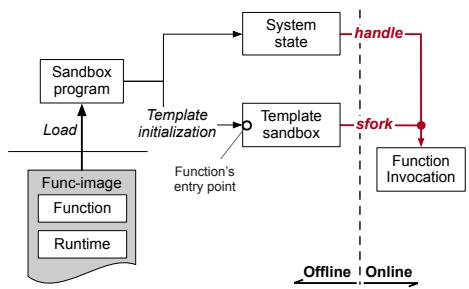
\includegraphics[width=\linewidth]{images/e7b2431a4d0f4e5dd65bc555bb413047bbb565e5cb86b54e9afa06dbda544023.jpg}
    \caption{沙箱 fork 概览。}
  \end{subfigure}\hfill
  \begin{subfigure}[t]{0.31\textwidth}
    \centering
    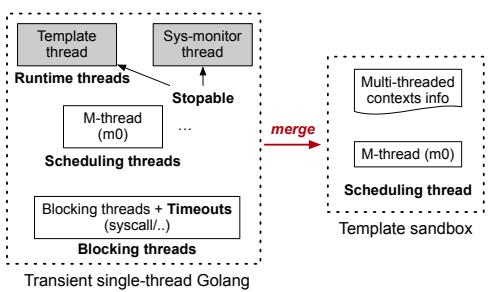
\includegraphics[width=\linewidth]{images/883cfb76a68135479e39415ffc29470bbf9b52476287290a5ab5948d8343e92d.jpg}
    \caption{面向 Go 的瞬时单线程机制。}
  \end{subfigure}\hfill
  \begin{subfigure}[t]{0.31\textwidth}
    \centering
    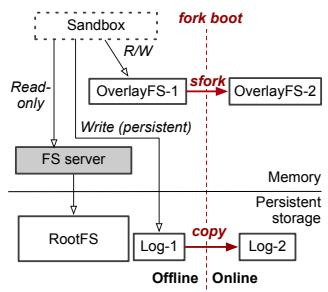
\includegraphics[width=\linewidth]{images/f19d4ce790aa02be4efbafd2b40449781c3203bb9639e1c52662c411375846b1.jpg}
    \caption{无状态 Overlay RootFS。}
  \end{subfigure}
  \caption{带有沙箱 fork 的 \sys{}。系统可离线生成模板沙箱，并在收到请求后通过 \emph{sfork} 派生新实例；瞬时单线程机制支持多线程程序的安全 fork；无状态 Overlay RootFS 使文件描述符和文件状态的处理变得高效。}
  \label{fig:sfork}
\end{figure*}

为保证一致性，\sys{} 尽量把不一致状态的修复放在用户态完成，只对内核做最小改动。
系统把沙箱中的系统调用分为三类：禁止（denied）、允许（allowed）和受控处理（handled）。
允许与受控处理的系统调用见 \tabref{tab:syscalls}；其中，受控处理的调用需要在 \emph{sfork} 后额外执行用户态修复逻辑，以恢复一致的系统状态。
例如，\texttt{clone} 会创建新的线程上下文，因此派生后的多线程上下文必须显式恢复。
禁止类系统调用则会被移出沙箱，以避免引入不可预测的系统状态变化。
\sys{} 通过两项新技术解决关键挑战：瞬时单线程机制负责恢复多线程上下文，无状态 Overlay RootFS 负责安全复用继承的文件描述符。
内核侧唯一新增的是共享内存映射上的 CoW 标志；而用户 ID、进程 ID 等状态则依赖 Linux 容器命名空间机制（USER/PID namespace）保持一致。

\subsection{多线程 fork}\label{sec:multithread-fork}
以 gVisor 为代表的 Go 实现沙箱天然是多线程的，因为 Go 运行时需要后台线程来完成垃圾回收、调度和其它运行时任务。
从语义上看，这些线程可以分为三类：运行时线程、调度线程以及阻塞线程，如 \figref{fig:sfork} 所示。
运行时线程负责垃圾回收、抢占等底层功能，通常对开发者透明；调度线程负责承载 Go 协程；当某个 Go 协程进入阻塞状态（例如执行 \texttt{accept}）时，Go 运行时会为其分配一个操作系统线程。

\sys{} 提出 \emph{瞬时单线程}（transient single-thread）机制，以支持多线程沙箱的 fork。
其核心思想是在派生前短暂地把一个多线程程序收敛为单线程，再在 \emph{sfork} 后把它重新扩展回多线程。
为此，我们修改了 Go 运行时，使运行时线程可以被暂停并将上下文保存到内存后主动退出；调度线程数可被临时收缩为 1；阻塞线程则设置超时，在超时时检查自己是否需要退出以进入单线程态。
最终，程序在模板生成时只保留 \texttt{m0} 线程，\emph{sfork} 完成后再恢复为多线程。
这一修改仅用于模板生成阶段，不影响 \emph{sfork} 之后的程序语义。

\subsection{无状态 Overlay RootFS}\label{sec:overlay-rootfs}
\emph{sfork} 得到的子沙箱会继承模板沙箱的文件描述符和文件系统状态，因此这些资源必须在派生后被正确处理。
受 OverlayFS~\cite{r13} 和 Serverless 函数短生命周期特征~\cite{r27,r28} 的启发，\sys{} 设计了 \emph{无状态 Overlay RootFS}，以近乎零成本地处理文件描述符和 rootfs。
其关键思想是把针对 rootfs 的所有修改都放在内存层完成，这些内存修改可在 \emph{sfork} 时自动通过写时复制克隆，如 \figref{fig:sfork} 所示。

具体地，每个沙箱使用两层文件系统。
上层是私有的内存态 OverlayFS，支持读写；其后端是一个按函数划分的 FS server，后者负责管理真实 rootfs。
为了安全，沙箱不能直接访问持久化存储，而是通过 FS server 发放的只读文件描述符访问底层 rootfs。
在 \emph{sfork} 过程中，模板沙箱拥有的只读文件描述符仍然可以安全地被子沙箱继承，因此大多数文件都能以极低开销完成复用。
工业实践还表明，有时 Serverless 函数确实需要访问少量持久化文件（例如日志文件）。
对此，\sys{} 允许 FS server 额外授予少量具有读写权限的日志文件描述符；总体上，绝大多数文件都能通过低时延复用完成，只有极少数必须持久化的文件需要显式复制。

\begin{table*}[t]
  \centering
  \small
  \begin{tabularx}{\textwidth}{p{1.6cm}p{2.5cm}X}
    \toprule
    类别 & 处理方式 & 相关系统调用 \\
    \midrule
    进程 & 瞬时单线程、命名空间保持一致 & \texttt{capget}, \texttt{clone}, \texttt{getpid}, \texttt{gettid}, \texttt{arch\_prctl}, \texttt{prctl}, \texttt{rt\_sigaction}, \texttt{rt\_sigprocmask}, \texttt{rt\_sigreturn}, \texttt{seccomp}, \texttt{sigaltstack}, \texttt{sched\_getaffinity} \\
    VFS（文件/网络） & 只读 FD 继承 & \texttt{poll}, \texttt{ioctl}, \texttt{memfd\_create}, \texttt{ftruncate}, \texttt{mount}, \texttt{pivot\_root}, \texttt{umount}, \texttt{epoll\_create1}, \texttt{epollCtl}, \texttt{epoll\_pwait}, \texttt{eventfd2}, \texttt{fcntl}, \texttt{chdir}, \texttt{close}, \texttt{dup}, \texttt{dup2}, \texttt{lseek}, \texttt{openat} \\
    文件（存储） & 无状态 OverlayFS & \texttt{newstat}, \texttt{newstatat}, \texttt{mkdirat}, \texttt{write}, \texttt{read}, \texttt{readlinkat}, \texttt{pread64} \\
    网络 & 按需重连 & \texttt{sendmsg}, \texttt{shutdown}, \texttt{recvmsg}, \texttt{getsockopt}, \texttt{listen}, \texttt{accept} \\
    内存 & 由 \emph{sfork} 处理 & \texttt{mmap}, \texttt{munmap} \\
    杂项 & 命名空间保持一致 & \texttt{setgid}, \texttt{setuid}, \texttt{get(e)gid}, \texttt{get(e)uid}, \texttt{getrandom}, \texttt{nanosleep}, \texttt{futex}, \texttt{getgroups}, \texttt{clock\_gettime}, \texttt{getrlimit}, \texttt{setsid} \\
    \bottomrule
  \end{tabularx}
  \caption{\sys{} 在 \emph{sfork} 中对系统调用的分类。普通字体表示允许但无需额外处理的系统调用；需要显式用户态修复逻辑的调用则归入“处理方式”一栏。}
  \label{tab:syscalls}
\end{table*}

\subsection{面向冷启动的语言运行时模板}\label{sec:runtime-template}
尽管按需恢复已经能提供相当优秀的冷启动性能，但它依赖包含未压缩数据的函数镜像，因此镜像体积更大。
为此，\sys{} 还提供了另一种冷启动路径：\emph{语言运行时模板}。
它本质上是针对同一语言的一类函数共享的模板沙箱：模板先完成语言运行时环境初始化（例如 Java 中的 JVM），请求到来后再按需加载真实函数。
不同语言的模板构造方式有所不同，例如 C 模板偏向预加载库文件，而 Java 模板则会预加载类文件。
在我们的工业环境中，由于大部分函数使用 Java 编写，单一 JVM 模板就足以为大量函数显著提速。

\section{实现}\label{sec:impl}
\sys{} 基于 gVisor 实现：其中对 gVisor 本身的修改约为 2017 行，对 Go 运行时为支持 \emph{sfork} 的修改约为 732 行；为了支持免初始化启动及各项优化，总计还加入了约 5000 行 Go 代码。
此外，我们扩展了平台侧基础设施，包括约 300 行 C 代码实现的内核模块以及约 500 行 Go 编写的用户态管理程序。

除本文设计中的核心技术外，\sys{} 还包含若干额外优化，以进一步压缩启动时延，例如更细粒度的函数入口点选择（\secref{sec:optimizations}）。
\figref{fig:boot-techniques} 汇总了这些技术在不同启动模式中的使用方式。

离线函数镜像编译过程如下：
(1) 将用户提供的函数入口点插入 wrapper 程序，作为注解；
(2) 编译时把该注解替换成一次系统调用，例如 C 语言通过 \texttt{libc} 的 \texttt{syscall()}，Java 则通过 JNI 调用；
(3) 包装程序开始运行，并在到达函数入口点时陷入 gVisor 内核；
(4) 系统把当前程序状态——包括内存数据、系统元数据以及 I/O 信息——一起保存进函数镜像。
整个流程大部分都可自动化完成。

虽然本文选择在 gVisor/Go 上实现 \sys{}，但其设计并不依赖于某一个特定系统。
例如，Firecracker 启动客体内核仍需要 100ms 以上，因此同样可以受益于按需恢复；而覆盖内存等技术只依赖 Intel EPT 或 AMD NPT 这类硬件虚拟化扩展。
此外，瞬时单线程机制也可迁移到其它基于 Go 的轻量虚拟化系统，例如 novm~\cite{r9}。

\begin{figure}[t]
  \centering
  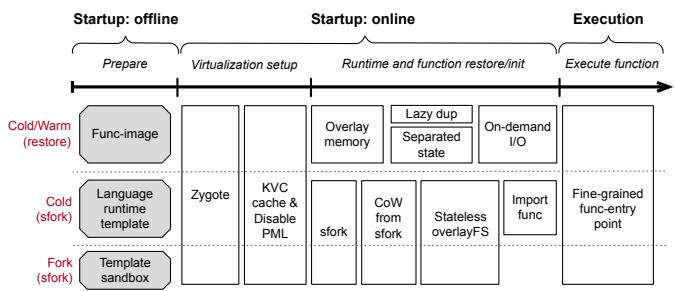
\includegraphics[width=\linewidth]{images/11f0b639eecfc937d672a87d3e16f319e8e5f8a24e7ad60e7ffe1479ee58ae24.jpg}
  \caption{\sys{} 在不同启动模式下采用的技术与优化手段。除 \secref{sec:ondemand-restore} 和 \secref{sec:sfork} 中的核心设计外，\sys{} 还通过更细粒度的函数入口点等工程优化进一步降低时延。}
  \label{fig:boot-techniques}
\end{figure}

\section{评估}\label{sec:eval}
评估围绕以下问题展开：
\begin{itemize}[leftmargin=1.2em]
  \item \textbf{问题 1：} \sys{} 对不同应用的启动性能提升有多大？
  \item \textbf{问题 2：} \sys{} 中的各项技术分别贡献了多少收益？
  \item \textbf{问题 3：} \sys{} 对真实 Serverless 工作负载的端到端时延改善如何？
  \item \textbf{问题 4：} \sys{} 对平台内存占用有何影响？
  \item \textbf{问题 5：} 当系统中存在大量并发实例时，\sys{} 的可扩展性如何？
  \item \textbf{问题 6：} \sys{} 是如何进一步逼近 1ms 启动时延的？
  \item \textbf{问题 7：} \sys{} 是否引入新的安全问题？
  \item \textbf{问题 8：} 工业部署带来了哪些经验教训？
\end{itemize}

\subsection{评估环境}\label{sec:eval-env}
我们使用一台实验机器进行微基准与性能分解评估：8 核 Intel i7-7700，32GB 内存，Samsung 512GB SSD，操作系统为 Ubuntu 16.04，内核版本 4.17.3。
此外，还使用蚂蚁金服的一台服务器进行端到端时延与扩展性评估，该服务器配备 96 个核心（2.50GHz）和 256GB 内存。
对比系统包括 gVisor（commit \#56fa562）、采用官方精简内核的 Firecracker（commit \#28f44b3）、Docker runc（commit \#bbb17ef）以及 Hyper Container（commit \#565496c）。

\subsection{应用启动时延}\label{sec:startup-latency}
\para{方法。}
我们比较三种 \sys{} 启动模式：冷启动（Catalyzer-restore）、温启动（Catalyzer-Zygote）与 fork 启动（Catalyzer-sfork），对比对象为 Docker、Hyper Container、gVisor、gVisor-restore 以及 Firecracker。
测试覆盖 C、Java、Python、Ruby 与 Node.js 五种语言。
每种语言都包含两个工作负载：一个最小应用 HelloWorld，一个真实应用。
由于 Firecracker 官方内核当时尚不支持 Ruby，因此该组合未纳入实验。
C 语言应用选用 Nginx 1.11.3，并以从执行 \texttt{nginx} 命令到其主函数开始的时间作为启动时延；Java 采用 SPECjbb2015，并测量从执行 \texttt{java} 到 \texttt{BackendAgent} 入口的时间；Python 使用 Django，Ruby 使用 Sinatra，Node.js 则使用一个 Web 服务器应用。

\begin{table}[t]
  \centering
  \small
  \begin{tabular}{lccc}
    \toprule
    系统 & 原生运行 & gVisor & Java 模板 \\
    \midrule
    冷启动时延（ms） & 89.4 & 659.1 & 29.3 \\
    \bottomrule
  \end{tabular}
  \caption{使用 Java 运行时模板进行冷启动的时延。}
  \label{tab:java-template}
\end{table}

\begin{figure*}[t]
  \centering
  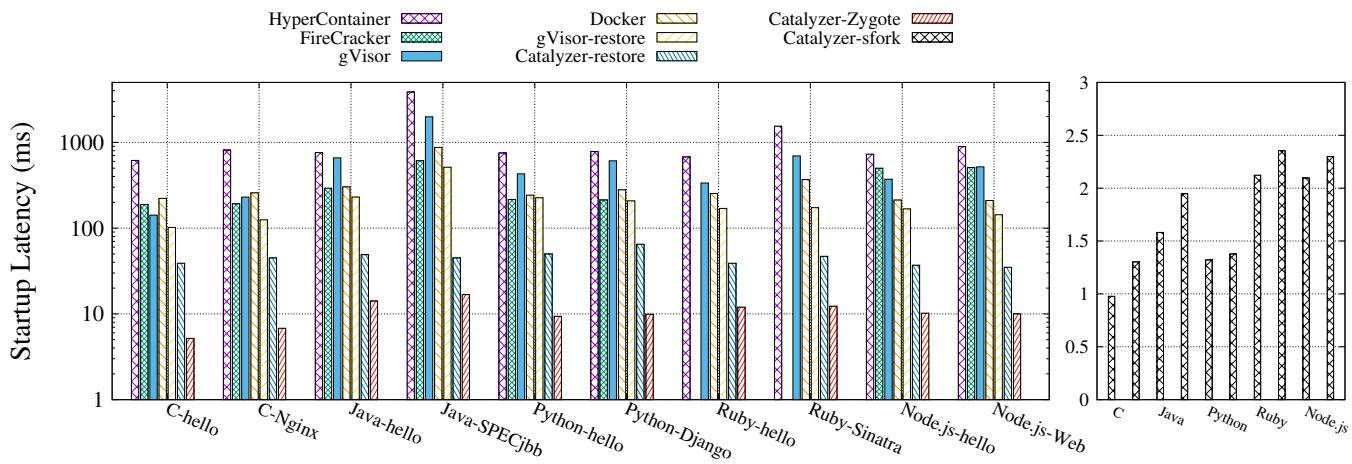
\includegraphics[width=0.92\textwidth]{images/eb7f755b975e5e4f9a4e74b39b0c82517565f9dbe99cfc855de2e6d79502c91f.jpg}
  \caption{\sys{} 与其它系统的启动时延对比。右半部分中的 Catalyzer-sfork 使用与左半部分相同的测试用例。}
  \label{fig:startup}
\end{figure*}

\para{结果。}
如 \figref{fig:startup} 所示，\sys{} 在所有应用上都取得了最佳性能。
其中，Catalyzer-sfork 在 C Hello 场景下把启动时延降到 0.97ms；Catalyzer-Zygote 在 C、Java、Python、Ruby 和 Node.js 场景中分别可把启动时延控制在约 5ms、14ms、9ms、12ms 和 9ms。
相较之下，Catalyzer-restore 通常比 Zygote 路径多出约 30ms，用于沙箱初始化和函数镜像映射。
这些结果表明，\sys{} 的收益具有很强的通用性：从最简单的 C Hello 到重量级的 Java SPECjbb 都能显著受益。

\para{语言运行时模板。}
虽然 \emph{sfork} 主要面向热启动，但结合 \secref{sec:runtime-template} 中的语言运行时模板，它也可以为同一语言的不同函数提供通用模板，从而为轻量函数带来快速冷启动。
如 \tabref{tab:java-template} 所示，使用 JVM 模板时，一个轻量级 Java 函数的冷启动时延只有 29.3ms，比基线 gVisor 快约 30 倍；甚至比原生启动还快 3.0--3.7 倍。
此时 \emph{sfork} 的主要剩余开销来自目标函数类文件的加载。

\subsection{收益分解}\label{sec:breakdown-eval}
为了评估各项技术的独立收益，我们以 gVisor-restore 为基线，在两类应用上进行分解实验：Python Django 与 Java SPECjbb。
比较的配置包括：原始 gVisor-restore、关闭“分离式装载”和“惰性 I/O 重连”的 \sys{}、仅关闭“惰性 I/O 重连”的 \sys{}，以及完整 \sys{}。

\begin{figure}[t]
  \centering
  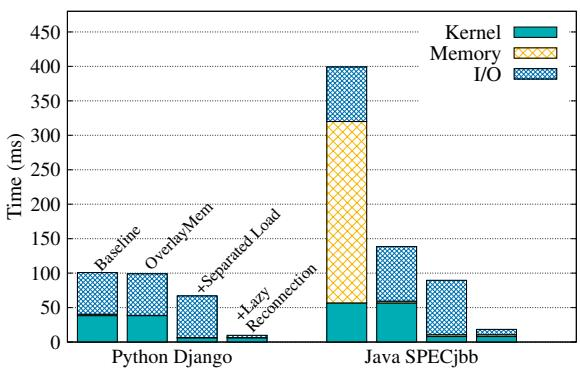
\includegraphics[width=\linewidth]{images/5f62973159daf055e47fd2f4f5bf01c628289c5a08147c2d69afc35be1c38dd4.jpg}
  \caption{\sys{} 冷启动路径的细粒度收益分解。}
  \label{fig:breakdown}
\end{figure}

如 \figref{fig:breakdown} 所示，覆盖内存相较 gVisor-restore 在 Java SPECjbb 上单独减少了 261ms 时延；分离式对象装载使内核对象装载时延在 Python Django 上降低了 6.3 倍，在 Java SPECjbb 上降低了 7.0 倍；惰性 I/O 重连则在两种应用中都减少了超过 57ms 的 I/O 重连时延，相当于约 18 倍提升。
总体而言，小内存应用从“分离式对象装载”和“惰性 I/O 重连”中受益更大，而大内存应用最显著的收益来自覆盖内存。

\subsection{端到端评估}\label{sec:e2e}
我们选取三类真实工作负载，展示 \sys{} 对端到端 Serverless 时延的改善效果。
在每个实验中，我们同时报告启动时延（Boot）与执行时延（Execution），并比较 gVisor、Catalyzer-sfork（fork 启动）以及 Catalyzer-restore（冷启动）三种路径。

\para{DeathStar 社交网络微服务。}
DeathStar 是一个开源微服务基准套件~\cite{r22}。
我们把其中 5 个社交网络微服务迁移到自研的 Serverless 平台中，并把微服务间调用替换为适配平台的 stub 函数。
如 \figref{fig:e2e} 中的子图 (a) 所示，这代表了一类轻量级真实 Serverless 工作负载。
所有函数都用 C++ 编写，执行时延在所有场景下都低于 2.5ms。
在这类函数上，\sys{} 主要通过压缩启动时延改善总时延：使用 \emph{sfork} 时，总体可提升 35--67 倍。

\para{图像处理应用。}
图像处理是 Serverless 的典型应用之一，也在已有平台上得到实践~\cite{r17}。
我们使用 Python Pillow 库~\cite{r15} 实现了五个典型图像处理任务：增强、滤镜、滚动、拆分/合并以及转置。
这些函数会接收图像、完成处理并返回结果。
如 \figref{fig:e2e} 中的子图 (b) 所示，其执行时延大约在 100--200ms 之间，主要成本来自输入图像读取。
虽然执行时间比 DeathStar 更长，但启动时延依然占据主导（通常超过 500ms）。
相较基线，\sys{} 在 fork 启动下可把端到端时延降低 4.1--6.5 倍，在冷启动下可降低 3.6--4.3 倍。

\para{电商函数。}
我们还评估了四个 Java 编写的电商 Serverless 函数：购买、广告投放、报表生成和折扣应用。
这些服务的执行时长从数百毫秒到一秒以上不等。
如 \figref{fig:e2e} 中的子图 (c) 所示，在基线 gVisor 中，这四个应用的启动阶段占据了其端到端时延的 34\%--88\%；而在 \sys{} 中，这一比例均降到 5\% 以下，已经能够满足大多数服务场景对启动成本的容忍要求。

\begin{figure*}[t]
  \centering
  \begin{subfigure}[t]{0.32\textwidth}
    \centering
    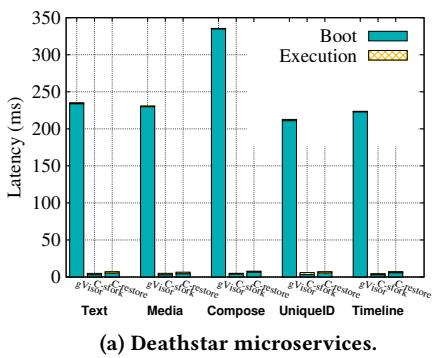
\includegraphics[width=\linewidth]{images/060915cf5c3801063931aac3c942646725df134d9fc029c924ea57357745f449.jpg}
    \caption{DeathStar 微服务。}
  \end{subfigure}\hfill
  \begin{subfigure}[t]{0.32\textwidth}
    \centering
    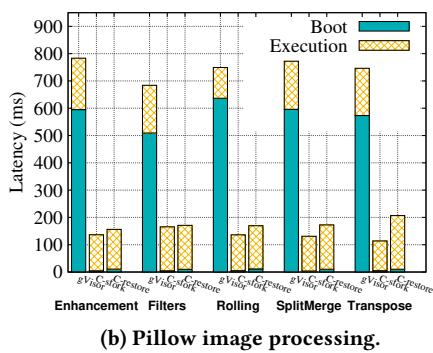
\includegraphics[width=\linewidth]{images/02ca13c54929d60cfe9bc999009ad8cb6f16433b10287e1cd42820ea513e5fbb.jpg}
    \caption{Python Pillow 图像处理。}
  \end{subfigure}\hfill
  \begin{subfigure}[t]{0.32\textwidth}
    \centering
    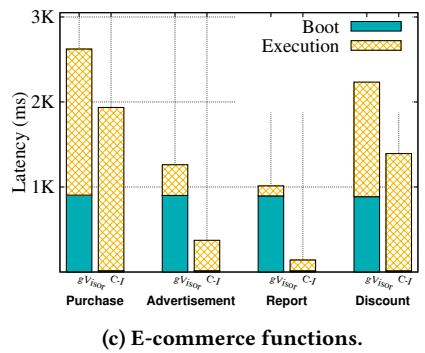
\includegraphics[width=\linewidth]{images/e47696e3dc8466b5939bcae14f9188ab6475208dbbef3d67585907fe83486b12.jpg}
    \caption{Java 电商函数。}
  \end{subfigure}
  \caption{端到端评估。图中 C-sfork 表示 \sys{} 的 fork 启动，C-restore 表示 \sys{} 的冷启动，C-I 表示在工业服务器环境中的 \sys{} 结果。}
  \label{fig:e2e}
\end{figure*}

\subsection{内存使用评估}\label{sec:memory}
\para{按需分页的内存收益。}
\figref{fig:memory} 比较了 DeathStar 中 \texttt{composePost} 函数在 gVisor 和带 \emph{sfork} 的 \sys{} 上的内存占用。
实验从 1 个并发实例增加到 16 个并发实例，分别使用 RSS（resident set size）和 PSS（proportional set size）衡量内存占用。
RSS 表示进程实际占用的总内存；PSS 则是“私有内存 + 共享内存按比例分摊”的总和。
图中每个点都是所有运行沙箱内存占用的平均值。
可以看到，相比 gVisor，\sys{} 在 RSS 和由 PSS 反映的私有内存上都更低，这说明其共享内存策略有效降低了实例间冗余。

\begin{figure*}[t]
  \centering
  \begin{subfigure}[t]{0.48\textwidth}
    \centering
    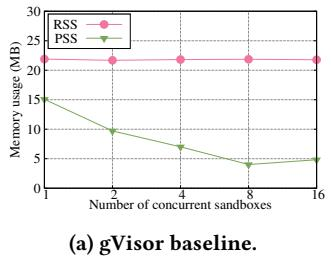
\includegraphics[width=\linewidth]{images/19c97f2c1754385d5e64fd5f2de3434914a355f40a62c66abef9433720412080.jpg}
    \caption{RSS。}
  \end{subfigure}\hfill
  \begin{subfigure}[t]{0.48\textwidth}
    \centering
    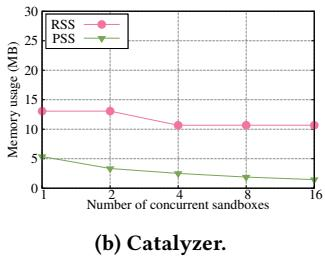
\includegraphics[width=\linewidth]{images/58190f206cfe0abc4f6bb80d8af4a42276941e9c7bffa4c9b1739a4b48fab1dc.jpg}
    \caption{PSS。}
  \end{subfigure}
  \caption{DeathStar 场景下的内存占用对比。}
  \label{fig:memory}
\end{figure*}

\para{\sys{} 的额外内存开销。}
\sys{} 温启动路径的内存额外开销是可接受的。
我们观察到，一部分元数据对象会被复制到 Private-EPT 中，形成额外的内存占用。
\tabref{tab:memory-cost} 给出了元数据对象与 I/O cache 的成本：I/O cache 通常不超过 2.4KB，而元数据对象开销在 165KB 到 680KB 之间。
重要的是，这一成本是“按函数”而不是“按实例”计的，因此总开销控制在 683KB 以内，对大多数场景来说是可以接受的。
当然，\emph{sfork} 会带来更高的模板内存占用，例如一个 SPECjbb 模板沙箱可能超过 200MB，但这主要用于热点函数的持续热启动。

\begin{table}[t]
  \centering
  \small
  \begin{tabular}{lrrr}
    \toprule
    应用 & 元数据对象 & I/O Cache & 总开销 \\
    \midrule
    C-Nginx & 165.5KB & 370B & 165.9KB \\
    Java-SPECjbb & 680.6KB & 2.4KB & 683.0KB \\
    Python-Django & 289.3KB & 1.2KB & 290.5KB \\
    Ruby-Sinatra & 349.2KB & 1.5KB & 350.8KB \\
    NodeJS-Web & 302.1KB & 472B & 302.6KB \\
    \bottomrule
  \end{tabular}
  \caption{\sys{} 在温启动中的额外内存成本。}
  \label{tab:memory-cost}
\end{table}

\subsection{并发运行}\label{sec:concurrent}
Serverless 的核心优势之一是自动扩缩容，因此单机上同时运行大量函数实例是常态。
我们使用 DeathStar 中的 \texttt{text} 服务作为测试函数；该函数在处理请求后会短暂挂起再退出，因此适合模拟并发场景。
如 \figref{fig:scaling} 所示，我们让同时运行的实例数从 0 增长到 1000，并比较 \sys{} 与 gVisor-restore。
对于 gVisor-restore，我们只统计恢复时延，不包含创建沙箱的额外时间。
结果表明，无论在实验机器还是工业服务器上，\sys{} 的启动时延始终低于 10ms，展现了良好的扩展性。

\begin{figure}[t]
  \centering
  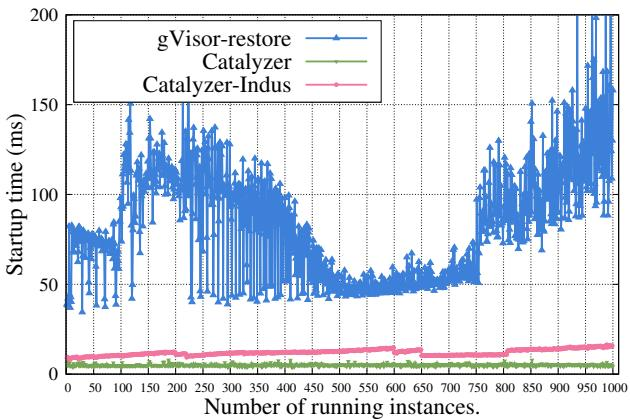
\includegraphics[width=\linewidth]{images/dc0d9b30ecebf3e5452ad8b13f2a6e2819176419b4296576866fdaa00831f7ad.jpg}
  \caption{随着并发实例数增加时的启动时延。Catalyzer-Indus 表示工业服务器上的结果。}
  \label{fig:scaling}
\end{figure}

\subsection{进一步优化}\label{sec:optimizations}
除核心设计外，\sys{} 还采用了若干工程优化，把启动时延进一步逼近 1ms。

\para{更细粒度的函数入口点。}
如果开发者能更仔细地选择函数入口点位置，例如把入口点后移到函数内部某段准备逻辑之后，那么还可以进一步压缩启动时延。
这样做的本质是把一部分与具体应用相关的准备工作也转移到离线阶段。
开发者需要确保这些被提前执行的状态不泄露用户隐私，也不会破坏安全语义。
平台甚至可以用用户提供的训练请求对某些依赖项进行预热，从而形成“用户引导的预初始化”状态。
我们在 Java SPECjbb 和一个内存访问型 C 微基准上验证了这一点；如 \figref{fig:optimizations} 中的子图 (a) 所示，两者执行时延都可进一步降低约 3 倍。

\para{KVM 优化。}
当前 KVM 默认开启页面修改日志（Page Modification Logging, PML），用于记录客体物理页的修改。
如果来宾实际上不需要这项功能，那么它会显著拖慢新增内存区域的延迟，如 \figref{fig:optimizations} 中的子图 (c) 所示。
因此，我们在基线与 \sys{} 中都默认关闭 PML，从而为设置 KVM 内存区域减少 5--8ms 时延。
此外，KVM 在为虚拟机管理分配内部数据结构时使用 \texttt{kvcalloc}，这一操作本身就可能带来约 1.6ms 开销。
我们为其增加了一个专用缓存，使绝大多数分配都能在 \(<50\,\mu s\) 内完成，如子图 (b) 所示。

\para{高尾时延系统调用。}
宿主机内核中的某些系统调用会表现出极高的尾时延。
例如，\texttt{dup}/\texttt{dup2} 的执行时间从不足 1ms 到 30ms 不等，如 \figref{fig:optimizations} 中的子图 (d) 所示。
这类突发时延通常来自内核中的稀有路径，例如文件描述符表扩容。
为缓解这一问题，我们实现了 \emph{lazy dup}：Gofer 进程先返回一个可用 FD 给客户端，再异步为自己复制出一个新的 FD。
这一优化被用于按需 I/O 重连路径，可额外贡献 10--20ms 改善。

\begin{figure*}[t]
  \centering
  \begin{subfigure}[t]{0.24\textwidth}
    \centering
    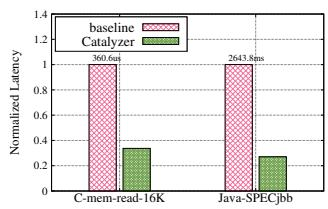
\includegraphics[width=\linewidth]{images/0092e4f63473ff81adfca8ec8d5cfff62af259f0b992960835d0c171972ee167.jpg}
    \caption{更细粒度的函数入口点。}
  \end{subfigure}\hfill
  \begin{subfigure}[t]{0.24\textwidth}
    \centering
    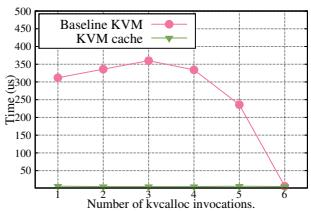
\includegraphics[width=\linewidth]{images/12a9ed1f8db0d4a3183e38e1bca0c3a129ffa7c94bd8ef3c6554a94b5f5f1f59.jpg}
    \caption{KVM 分配缓存。}
  \end{subfigure}\hfill
  \begin{subfigure}[t]{0.24\textwidth}
    \centering
    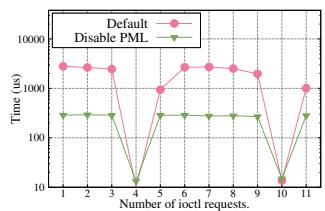
\includegraphics[width=\linewidth]{images/539432357dcf693650d5c01082be021b8407dd46f83b68946b4ca068f914083a.jpg}
    \caption{\texttt{set\_memory\_region} 的时延。}
  \end{subfigure}\hfill
  \begin{subfigure}[t]{0.24\textwidth}
    \centering
    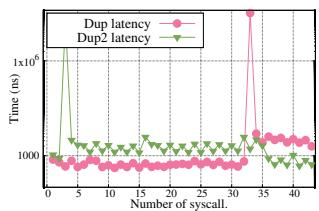
\includegraphics[width=\linewidth]{images/1020056c8496c78a993a335a36145a94b458d0e48bda7e7dcb84af435d160e99.jpg}
    \caption{\texttt{dup}/\texttt{dup2} 的时延。}
  \end{subfigure}
  \caption{\sys{} 中的工程优化。更细粒度的函数入口点可把应用相关准备工作前移，从而额外降低时延；为 KVM 增加缓存可显著减少 \texttt{kvcalloc} 开销；关闭 PML 可把 \texttt{\_\_ioctl\_set\_memory\_region} 的延迟降低约一个数量级；惰性 \texttt{dup} 则用于缓解少数宿主机系统调用的高尾时延。}
  \label{fig:optimizations}
\end{figure*}

\subsection{安全性分析}\label{sec:security}
\sys{} 会在多个实例之间共享一份“基础映射”（base mapping）。
由于该映射仅包含与用户请求无关的初始化状态，因此这种共享不会直接泄露用户数据，也不会额外引入新的缓存侧信道。
一个潜在问题是地址空间布局随机化（ASLR）被弱化：共享基础映射会降低布局的随机性。
对此，可以通过定期更新函数镜像与模板沙箱，或者采用已有的运行时重新随机化技术~\cite{r33,r34}，在 \emph{sfork} 过程中重新打乱地址空间布局。

\subsection{工业落地经验}\label{sec:lessons}
\para{重量级函数正在变得普遍。}
以往很多 Serverless 工作主要关注 Python 这类轻量级语言函数，但实际趋势是越来越多经长期打磨的 Java 服务代码被直接迁移为函数。
因此，一个能显著改善重量级语言运行时启动时延的系统非常必要。
近期针对 Java Serverless 启动加速的工作也从侧面验证了这一点~\cite{r43}。

\para{可持续的热启动。}
多数现有平台依赖函数缓存提供“热启动”，但其收益高度依赖缓存策略，并且无法改善由缓存未命中主导的尾时延。
\sys{} 基于 \emph{sfork} 的 fork 启动能够为热点函数提供一种更可持续的热启动能力。
当然，\emph{sfork} 的使用仍需结合工作负载与平台形态来决定。
在私有 Serverless 平台中，平台可以为不同函数赋予不同优先级，从而优先为高价值函数维持模板沙箱；在公有平台中，则需要开发者提供一定提示，以帮助平台更合理地决定何时切换到 fork 启动策略。

\section{相关工作}\label{sec:related}
除 \secref{sec:breakdown} 中讨论的系统外，还有一些工作尝试利用检查点/恢复机制加速实例化~\cite{r30,r42,r43}。
Potemkin 这类“闪克隆”系统利用一个包含预初始化 OS 与应用快照的参考镜像来快速克隆；SnowFlock~\cite{r30} 则通过虚拟机 fork 实现快速 VM 实例化。
但这些系统面向的是传统虚拟机，克隆时延仍较高，例如 SnowFlock 的 VM 克隆通常接近秒级。
Replayable Execution~\cite{r43} 将 FaaS 应用划分为两个执行阶段，并配合按需分页把 JVM 启动时延压到 54ms。
与之相比，\sys{} 有两点关键区别：第一，按需分页本身不足以解决虚拟化沙箱中的系统状态恢复问题，因此 \sys{} 同时对系统状态采用按需恢复；第二，\sys{} 进一步提出了 \emph{sfork}，使 Java 函数启动时延进入 1.5--2ms 量级。

另一类相关工作是 unikernel，例如 Mirage 与 OSv~\cite{r36,r26}。
它们通过最小化客体 OS、弱化应用与内核之间的隔离来获得比传统虚拟机更快的启动。
LightVM~\cite{r37} 通过优化 Xen 并最小化客体环境，可把 unikernel 启动压到 10ms 以内。
\sys{} 的思路与之不同：它不是继续缩短初始化，而是直接跳过初始化，因此对 Serverless 场景更高效；同时，我们也认为 \sys{} 的思想同样可以应用到 unikernel 生态中。

\section{结论}\label{sec:conclusion}
本文提出了 \sys{}：一种面向 Serverless 的通用启动加速设计。
它通过按需恢复与新的 \emph{sfork} 原语把初始化移出关键路径，从根本上消除了函数启动的主要成本。
我们在 gVisor 上完成实现，并通过多种语言、多类真实应用以及工业环境评估表明，\sys{} 能显著降低多样化 Serverless 应用的启动与端到端时延。

\section*{致谢}
感谢 shepherd Mike Swift 以及匿名审稿人提供的宝贵意见。
本工作得到国家重点研发计划（No.~2016YFB1000104）、国家自然科学基金（No.~61972244、61925206）、上海市科委高新技术支撑计划（No.~19511121100）以及上海市学术/技术带头人计划（No.~19XD1401700）的部分支持。
Yubin Xia（xiayubin@sjtu.edu.cn）为本文通信作者。

\small
\begin{thebibliography}{99}

\bibitem{r1} {[}n.d.{]}. Apache OpenWhisk is a serverless, open source cloud platform. http://openwhisk.apache.org/. Referenced December 2018.

\bibitem{r2} {[}n.d.{]}. AWS Lambda - Serverless Compute. https://aws.amazon.com/ lambda/. Referenced December 2018.

\bibitem{r3} {[}n.d.{]}. Azure Functions Serverless Architecture. https://azure.microsoft.com/en-us/services/functions/. Referenced December 2018.

\bibitem{r4} {[}n.d.{]}. Checkpoint/Restore in gVisor. https://gvisor.dev/docs/user\_guide/checkpoint\_restore/. Referenced July 2019.

\bibitem{r5} {[}n.d.{]}. The Docker Containerization Platform. https://www.docker.com/. Referenced December 2018.

\bibitem{r6} {[}n.d.{]}. Firecracker. https://firecracker-microvm.github.io/. Referenced December 2018.

\bibitem{r7} {[}n.d.{]}. Google Cloud Function. https://cloud.google.com/functions/. Referenced December 2018.

\bibitem{r8} {[}n.d.{]}. Google gVisor: Container Runtime Sandbox. https://github.com/google/gvisor. Referenced December 2018.

\bibitem{r9} {[}n.d.{]}. google/novm: Experimental KVM-based VMM for containers, written in Go. https://github.com/google/novm. Referenced Jan 2020.

\bibitem{r10} {[}n.d.{]}. Hyper - Make VM run like Container. https://hypercontainer.io/. Referenced December 2018.

\bibitem{r11} {[}n.d.{]}. Keeping Functions Warm - How To Fix AWS Lambda Cold Start Issue. https://serverless.com/blog/keep-your-lambdas-warm/. Referenced July 2019.

\bibitem{r12} {[}n.d.{]}. OCI Runtime Specification. https://github.com/opencontainers/runtime-spec. Referenced December 2018.

\bibitem{r13} {[}n.d.{]}. Overlay Filesystem. https://www.kernel.org/doc/ Documentation/filesystems/overlayfs.txt. Referenced July 2019.

\bibitem{r14} {[}n.d.{]}. Overview of memory management \textbar{} Android Developers. https://developer.android.com/topic/performance/memory-overview. Referenced December 2018.

\bibitem{r15} {[}n.d.{]}. Pillow: the friendly PIL fork. https://python-pillow.org/. Referenced December 2018.

\bibitem{r16} {[}n.d.{]}. Protocol Buffers Google Developers. https://developers.google.com/protocol-buffers/. Referenced July 2019.

\bibitem{r17} Istemi Ekin Akkus, Ruichuan Chen, Ivica Rimac, Manuel Stein, Klaus Satzke, Andre Beck, Paarijaat Aditya, and Volker Hilt. 2018. \{SAND\}: Towards High-Performance Serverless Computing. In 2018 \{USENIX\} Annual Technical Conference (\{USENIX\} \{ATC\} 18). 923--935.

\bibitem{r18} Nadav Amit and Michael Wei. 2018. The Design and Implementation of Hyperupcalls. In 2018 USENIX Annual Technical Conference (USENIX ATC 18). USENIX Association, Boston, MA, 97--112. https://www. usenix.org/conference/atc18/presentation/amit

\bibitem{r19} Adam Belay, Andrea Bittau, Ali José Mashtizadeh, David Terei, David Mazières, and Christos Kozyrakis. 2012. Dune: Safe User-level Access to Privileged CPU Features.. In Osdi, Vol. 12. 335--348.

\bibitem{r20} Fabrice Bellard. 2005. QEMU, a fast and portable dynamic translator.. In USENIX Annual Technical Conference, FREENIX Track, Vol. 41. 46.

\bibitem{r21} Sol Boucher, Anuj Kalia, David G. Andersen, and Michael Kaminsky. 2018. Putting the ``Micro'' Back in Microservice. In 2018 USENIX Annual Technical Conference (USENIX ATC 18). USENIX Association, Boston, MA, 645--650. https://www.usenix.org/conference/atc18/presentation/ boucher

\bibitem{r22} Yu Gan, Yanqi Zhang, Dailun Cheng, Ankitha Shetty, Priyal Rathi, Nayan Katarki, Ariana Bruno, Justin Hu, Brian Ritchken, Brendon Jackson, et al.~2019. An Open-Source Benchmark Suite for Microservices and Their Hardware-Software Implications for Cloud \& Edge Systems. In Proceedings of the Twenty-Fourth International Conference on Architectural Support for Programming Languages and Operating Systems. ACM, 3--18.

\bibitem{r23} Abel Gordon, Nadav Amit, Nadav Har'El, Muli Ben-Yehuda, Alex Landau, Assaf Schuster, and Dan Tsafrir. 2012. ELI: Bare-metal Performance for I/O Virtualization. In Proceedings of the Seventeenth International Conference on Architectural Support for Programming Languages and Operating Systems (ASPLOS XVII). ACM, New York, NY, USA, 411--422. https://doi.org/10.1145/2150976.2151020

\bibitem{r24} Joseph M Hellerstein, Jose Faleiro, Joseph E Gonzalez, Johann Schleier-Smith, Vikram Sreekanti, Alexey Tumanov, and Chenggang Wu. 2018. Serverless Computing: One Step Forward, Two Steps Back. arXiv preprint arXiv:1812.03651 (2018).

\bibitem{r25} Sanidhya Kashyap, Changwoo Min, and Taesoo Kim. 2018. Scaling Guest OS Critical Sections with eCS. In 2018 USENIX Annual Technical Conference (USENIX ATC 18). USENIX Association, Boston, MA, 159-- 172. https://www.usenix.org/conference/atc18/presentation/kashyap

\bibitem{r26} Avi Kivity, Dor Laor Glauber Costa, and Pekka Enberg. 2014. OS v---Optimizing the Operating System for Virtual Machines. In Proceedings of USENIX ATC'14: 2014 USENIX Annual Technical Conference. 61.

\bibitem{r27} Ana Klimovic, Yawen Wang, Christos Kozyrakis, Patrick Stuedi, Jonas Pfefferle, and Animesh Trivedi. 2018. Understanding Ephemeral Storage for Serverless Analytics. In 2018 USENIX Annual Technical Conference (USENIX ATC 18). USENIX Association, Boston, MA, 789-- 794. https://www.usenix.org/conference/atc18/presentation/klimovicserverless

\bibitem{r28} Ana Klimovic, Yawen Wang, Patrick Stuedi, Animesh Trivedi, Jonas Pfefferle, and Christos Kozyrakis. 2018. Pocket: Elastic Ephemeral Storage for Serverless Analytics. In 13th USENIX Symposium on Operating Systems Design and Implementation (OSDI 18). USENIX Association, Carlsbad, CA, 427--444. https://www.usenix.org/conference/osdi18/ presentation/klimovic

\bibitem{r29} Yossi Kuperman, Eyal Moscovici, Joel Nider, Razya Ladelsky, Abel Gordon, and Dan Tsafrir. 2016. Paravirtual Remote I/O. In Proceedings of the Twenty-First International Conference on Architectural Support for Programming Languages and Operating Systems (ASPLOS '16). ACM, New York, NY, USA, 49--65. https://doi.org/10.1145/2872362.2872378

\bibitem{r30} Horacio Andrés Lagar-Cavilla, Joseph Andrew Whitney, Adin Matthew Scannell, Philip Patchin, Stephen M Rumble, Eyal De Lara, Michael Brudno, and Mahadev Satyanarayanan. 2009. SnowFlock: rapid virtual machine cloning for cloud computing. In Proceedings of the 4th ACM European conference on Computer systems. ACM, 1--12.

\bibitem{r31} David Lion, Adrian Chiu, Hailong Sun, Xin Zhuang, Nikola Grcevski, and Ding Yuan. 2016. Don't Get Caught in the Cold, Warm-up Your JVM: Understand and Eliminate JVM Warm-up Overhead in Data-Parallel Systems. In 12th USENIX Symposium on Operating Systems Design and Implementation (OSDI 16). USENIX Association, Savannah, GA, 383--400. https://www.usenix.org/conference/osdi16/technicalsessions/presentation/lion

\bibitem{r32} Ming Liu, Simon Peter, Arvind Krishnamurthy, and Phitchaya Mangpo Phothilimthana. 2019. E3: Energy-Efficient Microservices on SmartNIC-Accelerated Servers. In 2019 USENIX Annual Technical Conference (USENIX ATC 19). USENIX Association, Renton, WA, 363--378. https://www.usenix.org/conference/atc19/presentation/liu-ming

\bibitem{r33} Kangjie Lu, Wenke Lee, Stefan Nürnberger, and Michael Backes. 2016. How to Make ASLR Win the Clone Wars: Runtime Re-Randomization.. In NDSS.

\bibitem{r34} Kangjie Lu, Chengyu Song, Byoungyoung Lee, Simon P Chung, Taesoo Kim, and Wenke Lee. 2015. ASLR-Guard: Stopping address space leakage for code reuse attacks. In Proceedings of the 22nd ACM SIGSAC Conference on Computer and Communications Security. ACM, 280--291.

\bibitem{r35} Anil Madhavapeddy, Thomas Leonard, Magnus Skjegstad, Thomas Gazagnaire, David Sheets, David J Scott, Richard Mortier, Amir Chaudhry, Balraj Singh, Jon Ludlam, et al.~2015. Jitsu: Just-In-Time Summoning of Unikernels.. In NSDI. 559--573.

\bibitem{r36} Anil Madhavapeddy, Richard Mortier, Charalampos Rotsos, David Scott, Balraj Singh, Thomas Gazagnaire, Steven Smith, Steven Hand, and Jon Crowcroft. 2013. Unikernels: Library operating systems for the cloud. In Acm Sigplan Notices, Vol. 48. ACM, 461--472.

\bibitem{r37} Filipe Manco, Costin Lupu, Florian Schmidt, Jose Mendes, Simon Kuenzer, Sumit Sati, Kenichi Yasukata, Costin Raiciu, and Felipe Huici. 2017. My VM is Lighter (and Safer) than your Container. In Proceedings of the 26th Symposium on Operating Systems Principles. ACM, 218--233.

\bibitem{r38} Garrett McGrath, Jared Short, Stephen Ennis, Brenden Judson, and Paul Brenner. 2016. Cloud event programming paradigms: Applications and analysis. In 2016 IEEE 9th International Conference on Cloud Computing (CLOUD). IEEE, 400--406.

\bibitem{r39} Edward Oakes, Leon Yang, Kevin Houck, Tyler Harter, Andrea C Arpaci-Dusseau, and Remzi H Arpaci-Dusseau. 2017. Pipsqueak: Lean Lambdas with large libraries. In 2017 IEEE 37th International Conference on Distributed Computing Systems Workshops (ICDCSW). IEEE, 395--400.

\bibitem{r40} Edward Oakes, Leon Yang, Dennis Zhou, Kevin Houck, Tyler Harter, Andrea Arpaci-Dusseau, and Remzi Arpaci-Dusseau. 2018. \{SOCK\}: Rapid Task Provisioning with Serverless-Optimized Containers. In 2018 \{USENIX\} Annual Technical Conference (\{USENIX\} \{ATC\} 18).

\bibitem{r41} Zhiming Shen, Zhen Sun, Gur-Eyal Sela, Eugene Bagdasaryan, Christina Delimitrou, Robbert Van Renesse, and Hakim Weatherspoon. 2019. X-containers: Breaking down barriers to improve performance and isolation of cloud-native containers. In Proceedings of the Twenty-Fourth International Conference on Architectural Support for Programming Languages and Operating Systems. ACM, 121--135.

\bibitem{r42} Michael Vrable, Justin Ma, Jay Chen, David Moore, Erik Vandekieft, Alex C Snoeren, Geoffrey M Voelker, and Stefan Savage. 2005. Scalability, fidelity, and containment in the potemkin virtual honeyfarm. In ACM SIGOPS Operating Systems Review, Vol. 39. ACM, 148--162.

\bibitem{r43} Kai-Ting Amy Wang, Rayson Ho, and Peng Wu. 2019. Replayable Execution Optimized for Page Sharing for a Managed Runtime Environment. In Proceedings of the Fourteenth EuroSys Conference 2019. ACM, 39.

\bibitem{r44} Liang Wang, Mengyuan Li, Yinqian Zhang, Thomas Ristenpart, and Michael Swift. 2018. Peeking behind the curtains of serverless platforms. In 2018 \{USENIX\} Annual Technical Conference (\{USENIX\} \{ATC\} 18). 133--146.

\bibitem{r45} Liang Zhang, James Litton, Frank Cangialosi, Theophilus Benson, Dave Levin, and Alan Mislove. 2016. Picocenter: Supporting Long-lived, Mostly-idle Applications in Cloud Environments. In Proceedings of the Eleventh European Conference on Computer Systems (EuroSys '16). ACM, New York, NY, USA, Article 37, 16 pages. https://doi.org/10. 1145/2901318.2901345

\end{thebibliography}

\end{document}
